% TEMPLATE for Usenix papers, specifically to meet requirements of
%  USENIX '05
% originally a template for producing IEEE-format articles using LaTeX.
%   written by Matthew Ward, CS Department, Worcester Polytechnic Institute.
% adapted by David Beazley for his excellent SWIG paper in Proceedings,
%   Tcl 96
% turned into a smartass generic template by De Clarke, with thanks to
%   both the above pioneers
% use at your own risk.  Complaints to /dev/null.
% make it two column with no page numbering, default is 10 point

% Munged by Fred Douglis <douglis@research.att.com> 10/97 to separate
% the .sty file from the LaTeX source template, so that people can
% more easily include the .sty file into an existing document.  Also
% changed to more closely follow the style guidelines as represented
% by the Word sample file. 

% Note that since 2010, USENIX does not require endnotes. If you want
% foot of page notes, don't include the endnotes package in the 
% usepackage command, below.

% This version uses the latex2e styles, not the very ancient 2.09 stuff.
% \documentclass[letterpaper,twocolumn,10pt]{article}
\pdfminorversion=4

\documentclass{hotnets15}

\usepackage{epsfig,endnotes}
\usepackage{color}
\usepackage{colortbl}
\usepackage{verbatim}
\usepackage[font=bf]{caption}
\usepackage{xspace}
\usepackage{mdframed}
\usepackage{float}
\usepackage{microtype}
\usepackage{newtxmath}

\usepackage{tikz}
\usepackage{enumitem}
\usepackage{booktabs}  % for toprule, bottomrule in tables
\usepackage[sort,space]{cite}
\usepackage{flushend}  % for balanced final columns


\usepackage{graphicx}
\usepackage{caption}
\usepackage{subfigure}

\newcommand{\subparagraph}{}
\usepackage[compact]{titlesec}

\usepackage{url}


\newcommand{\tightcaption}[1]{\vspace{-0.3cm}\caption{#1}\vspace{-0.3cm}}
\newcommand{\tightsection}[1]{\section{#1}}
\newcommand{\tightsubsection}[1]{\subsection{#1}}
\newcommand{\tightsubsubsection}[1]{\subsubsection{#1}}

\newcommand{\eg}{{\it e.g.,}\xspace}
\newcommand{\ie}{{\it i.e.,}\xspace}

\newcounter{note}[section]
\renewcommand{\thenote}{\thesection.\arabic{note}}

\newcommand{\Section}{\S}

\usepackage{pifont}
\newcommand{\cmark}{\ding{51}}%
\newcommand{\xmark}{\ding{55}}%

\newcommand{\fillme}{{\bf XXX}~}

\definecolor{purple}{RGB}{175,0,255}


\newcommand{\mypara}[1]{\medskip\noindent{\bf {#1}:}~}
\newcommand{\myparatight}[1]{\smallskip\noindent{\bf {#1}:}~}
\newcommand{\myparaq}[1]{\smallskip\noindent{\bf {#1}?}~}
\newcommand{\mysubparatight}[1]{\noindent {\it {#1}:}~}

%-- place any standard commands/environments here to get included in
%-- documents.  When you include this file, you should do it before
%-- the \begin{document} tag.

%%%%%%%%%%%%%%%%%%%%%%%%%%%%%%%%%%%%%%%%%%%%%%%%%%%%%%%%%%%%%%%%%%%%%%
%-- CHANGES:
%-- 07/31/01 -jstrunk- Added command to set the paper margins.

%-- Provides fixed width font for commands and code snips.
\newcommand{\code}[1]{\texttt{\textbf{#1}}}

%-- Terms...  Use this to introduce a term in the paper.
\newcommand{\term}[1]{\emph{#1}}

%-- Provides stylization for e-mail addresses
%\newcommand{\email}[1]{\emph{(#1)}}

%-- Starts a minor section (puts the title inline w/ the text.
\newcommand{\minorsection}[1]{\textbf{#1}:}

%-- Jiri caption
\newcommand{\minicaption}[2]{\caption[#1]{\textbf{#1.} #2}}

%-- Units on numbers: 4KB -> \units{4}{KB}
\newcommand{\units}[2]{#1~#2}

%-- Commands...  i.e. WRITE commands.
\newcommand{\command}[1]{{\sc \MakeLowercase{#1}}}

%-- For notes about things that need to be fixed.
\newcommand{\fix}[1]{\marginpar{\LARGE\ensuremath{\bullet}}
    \MakeUppercase{\textbf{[#1]}}}
%-- For adding inline notes to a draft preceded by your initials
%-- E.g., \fixnote{JJW}{What the heck is a foobar?}
\newcommand{\fixnote}[2]{\marginpar{\LARGE\ensuremath{\bullet}}
    {\textbf{[#1:} \textit{#2\,}\textbf{]}}}

%-- Setting margins: \setmargins{left}{right}{top}{bottom}
\newcommand{\setmargins}[4]{
    % Calculations of top & bottom margins
    \setlength\topmargin{#3}
    \addtolength\topmargin{-.5in}  %-- seems like this should be 1, but .5
                                   %-- balances the text top to bottom
    \addtolength\topmargin{-\headheight}
    \addtolength\topmargin{-\headsep}
    \setlength\textheight{\paperheight}
    \addtolength\textheight{-#3}
    \addtolength\textheight{-#4}

    % Calculations of left & right margins
    \setlength\oddsidemargin{#1}
    \addtolength\oddsidemargin{-1in}
    \setlength\evensidemargin{\oddsidemargin}
    \setlength\textwidth{\paperwidth}
    \addtolength\textwidth{-#1}
    \addtolength\textwidth{-#2}
}

%-- For the tabularx environment... Using L, C, R as the column type
%-- will left, center, or right justify the text.
\newcolumntype{L}{X}
\newcolumntype{C}{>{\centering\arraybackslash}X}
\newcolumntype{R}{>{\raggedleft\arraybackslash}X}

%-- To comment out a swatch of text, use \omitit{blah blah blah}
\long\def\omitit#1{}

%-- Inline title; useful for sub-sub-sections in which you don't want a separate
%-- line for the title.
\newcommand{\inlinesection}[1]{\smallskip\noindent{\textbf{#1.}}}


%%%
%%% COMMENTS / TODOS
%%%
\usepackage{ifthen}
\usepackage{xcolor}
\newcommand{\exclude}[1]{}
\newcommand{\showComments}{yes}
\newcommand{\note}[2]{
    \ifthenelse{\equal{\showComments}{yes}}{\textcolor{#1}{#2}}{}
}
\newcommand{\TODO}[1]{%
	\addcontentsline{tdo}{todo}{\protect{#1}}%
	\note{red}{TODO: #1}
}

\makeatletter \newcommand{\listoftodos}
{\section*{Todo List} \@starttoc{tdo}}
\newcommand{\l@todo}
{\@dottedtocline{1}{0em}{2.3em}} \makeatother


\newcommand{\myparaittight}[1]{\smallskip\noindent{\emph {#1}:}~}
\newcommand{\question}[1]{\smallskip\noindent{\emph{Q:~#1}}\smallskip}
\newcommand{\myparaqtight}[1]{\smallskip\noindent{\bf {#1}}~}
\newcommand{\jc}[1]{\note{green}{[HZ: #1]}}
\newcommand{\matt}[1]{\note{blue}{[MKM: #1]}}
\newcommand{\srini}[1]{\note{magenta}{[SS: #1]}}
\newcommand{\bruce}[1]{\note{red}{[BMM: #1]}}
\newcommand{\nadi}[1]{\note{purple}{[INB: #1]}}
\newcommand{\mycomment}[1]{}

\newcounter{packednmbr}

\newenvironment{packedenumerate}{\begin{list}{\thepackednmbr.}{\usecounter{packednmbr}\setlength{\itemsep}{0.5pt}\addtolength{\labelwidth}{-4pt}\setlength{\leftmargin}{\labelwidth}\setlength{\listparindent}{\parindent}\setlength{\parsep}{1pt}\setlength{\topsep}{0pt}}}{\end{list}}

\newenvironment{packeditemize}{\begin{list}{$\bullet$}{\setlength{\itemsep}{0.5pt}\addtolength{\labelwidth}{-4pt}\setlength{\leftmargin}{\labelwidth}\setlength{\listparindent}{\parindent}\setlength{\parsep}{1pt}\setlength{\topsep}{0pt}}}{\end{list}}


%
\def\sharedaffiliation{%
\end{tabular}
\begin{tabular}{c}}
%

\begin{document}

\title{Characterizing Reconfigurable Topologies in Datacenter Fabrics}

\numberofauthors{1}
\author{\alignauthor Paper \#16, 7 pages}


\maketitle



\subsection*{Abstract} 

\section{Introduction}
\label{sec:intro}

%% Maybe use some of this from SOLSTICE?
%% Today's datacenters aggregate tremendous amounts of compute and storage
%% capacity, driving demand for network switches with ever-increasing port counts
%% and line speeds.  However, supporting these demands with existing packet
%% switching technology is becoming increasingly expensive---in cost, heat, power,
%% and cabling. Packet switches are flexible, capable of making forwarding
%% decisions at the granularity of individual packets.  In common modern scenarios,
%% however, this flexibility is unnecessary: many (often consecutive) packets are
%% sent to the same output port.  Two key factors contribute to this traffic
%% pattern. First, traffic inside a datacenter often has high spatial locality,
%% where a large fraction of the traffic that enters each switch port is destined
%% for only a small number of output ports~\cite{msft-imc09, facebook:sigcomm15}.
%% Second, traffic is often bursty, with significant temporal locality between
%% packets sharing the same destination~\cite{bullet:conext13,
%%   facebook:sigcomm15}. The consequence of these two factors is that the traffic
%% demand matrix at a datacenter switch is often both skewed and
%% sparse~\cite{mordia:hotnets12,flyways,augmenting-dc-wireless}.

%% \begin{figure*}[t!!!]
%% \centering
%% 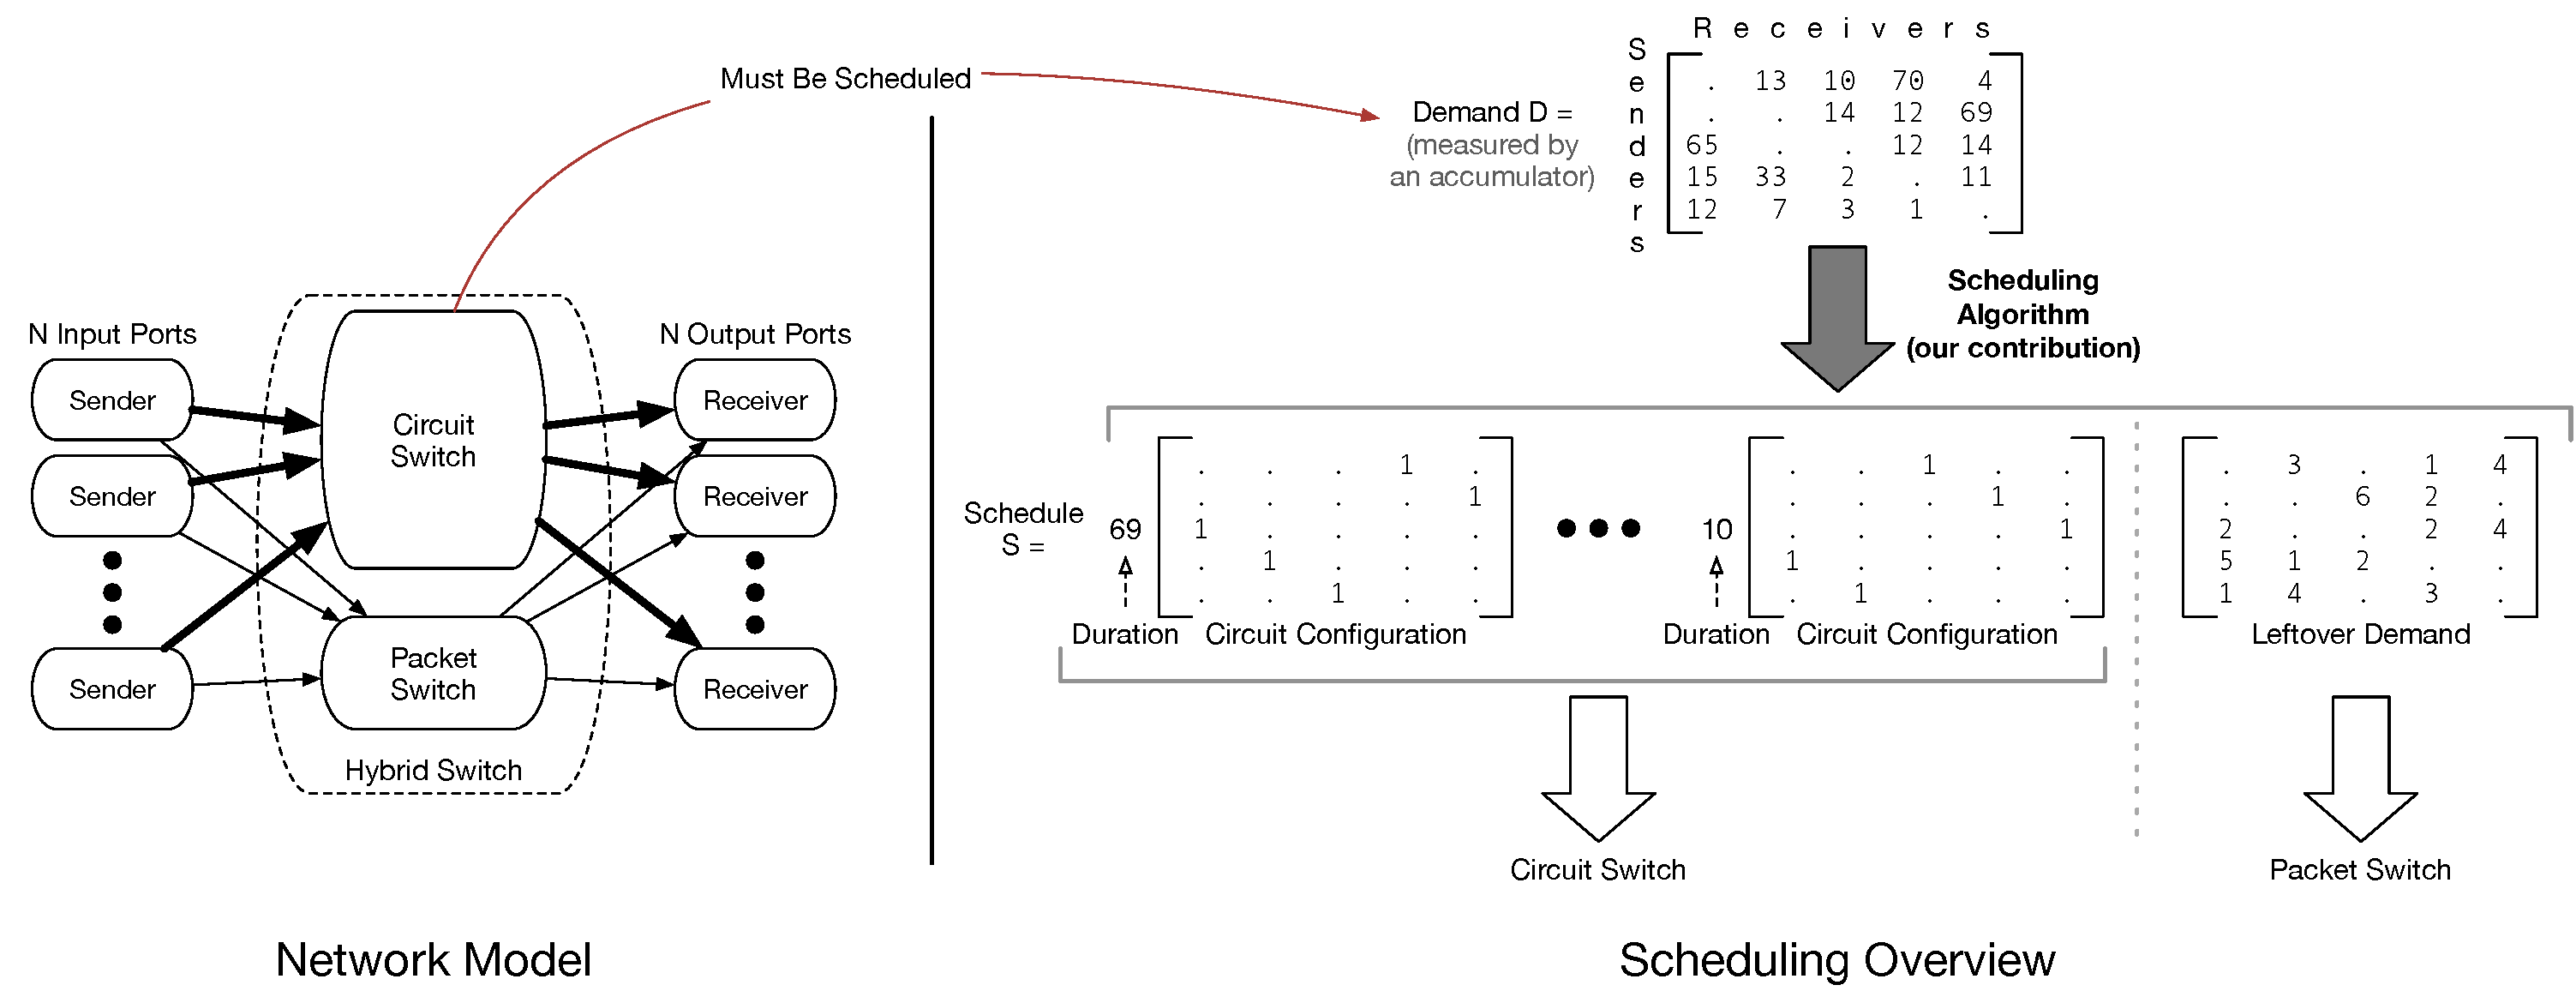
\includegraphics[width=1\textwidth]{figures/setting}
%% \caption{Our model of a hybrid switch architecture and the scheduling
%%   process. The circuit switch has high bandwidth, but slow reconfiguration
%%   time. The packet switch has low bandwidth (e.g., an order of magnitude lower),
%%   but can make forwarding decisions per-packet.
%%   %Both switches must have high utilization.
%%   }
%% \label{fig:arch}
%% \end{figure*}

%% Researchers have seized upon these observations to propose hybrid datacenter
%% network architectures that offer higher throughput at lower cost by combining
%% high-speed optical~\cite{OSA,helios:sigcomm10,c-Through} or
%% wireless~\cite{flyways,augmenting-dc-wireless,mirror-mirror} circuit switching
%% technologies with traditional electronic packet switches. Typically, the circuit
%% switch has a significantly higher data rate than the packet switch, but incurs a
%% non-trivial reconfiguration penalty. While the potential cost savings that
%% hybrid techniques could realize is large, the design space of scheduling
%% algorithms that enable high utilization in hybrid networks is not yet well
%% understood. Earlier work that considers circuit switches with substantial
%% reconfiguration delay offers no guidance about how to negotiate the trade-off
%% between remaining in the current (potentially sub-optimal) circuit configuration
%% vs. incurring a costly reconfiguration delay to switch to a potentially better
%% circuit configuration~\cite{c-Through, helios:sigcomm10, wang:hotnets}.  The
%% reconfiguration cost of these systems was so high that they were forced to keep
%% a configuration pinned up for a relatively long period anyway.

%% In recent years, however, the switching time of optical circuit switches has
%% improved substantially~\cite{mordia:sigcomm13}. As a result, an efficient
%% scheduling algorithm for a modern hybrid design must determine: 1) a set of
%% circuit configurations (which ports are connected to which other ports and how
%% long that configuration should remain in effect) designed to maximize the
%% traffic serviced over the high-bandwidth but slow-to-reconfigure
%% circuit-switched network, and 2) what traffic should be sent to the
%% low-bandwidth but flexible packet switch.

%% Computing an optimal set of circuit configurations to maximize circuit-switched
%% utilization has no known polynomial-time algorithms, scaling as $O(n!)$ in the
%% number of switch ports (\S\ref{sec:optimization}). The challenge arises due to
%% the non-trivial switching time between configurations, which necessitates not
%% only sending as much traffic as possible, but doing so in the fewest number of
%% configurations.

%% The end goal of this paper is an effective and fast heuristic algorithm that
%% delivers high switch utilization. To this end, we first provide a detailed
%% characterization of the problem plus an optimal (but impractical) solution that
%% sheds light on how to design an effective heuristic.  We then present our
%% heuristic, Solstice, which provides 2.9$\times$ higher utilization compared to
%% previous algorithms by taking advantage of the known sparsity and skew of
%% datacenter workloads---some of the same features that make the traditional
%% scheduling problem hard.

%% The contributions of this work are as follows:
%% \begin{enumerate}
%% \item Characterizing the hybrid switch scheduling problem.
%% \item Exploring the design space of hybrid scheduling:
%%   \begin{packedenumerate}
%%     \item \myparatight{Lower bound} an instantly computable but loose bound on
%%       the minimum amount of time it takes to serve all demand (but provides no
%%       actual schedules).
%%     \item \myparatight{Optimal scheduling} optimally schedule all
%%       demand with minimal time; impossible to run in real time at scale.
%%     \item \myparatight{Heuristic algorithm (``Solstice'')} runs in real time at
%%       scale, but slightly underperforms optimal (by at most 14\%
%%       at target scale).
%%     \item \myparatight{Heuristic + optimization (``\mbox{Solstice{}++}'')} runs at
%%       scale (though not in real time), but tightens the gap between Solstice and
%%       optimal (at most 12\% from optimal at target scale).
%%   \end{packedenumerate}
%% \item Insight into the challenges and benefits of using hybrid switches, with a
%%   focus on high circuit utilization.
%% \end{enumerate}

\begin{figure*}[t]
  \centering
  \begin{tabular}{| l | c | c | c | c | c | c |}
    \toprule
    & Bandwidth & Reconfig. Delay & Multicast & Comm. Paradigm & Packet Switch\\
    \midrule
    MSWL & & & & &\\
    ESWL & & & & &\\
    FSO & & & & &\\
    OCS & & & & &\\
    OCS-MC & & & & &\\
    \bottomrule
  \end{tabular}
  \caption{Examination of prior work.}
  \label{tab:prior}
\end{figure*}

\newpage\phantom{t}
\newpage



\section{Background}
\label{sec:background}

\subsection{Model}
\label{sec:model}

{\bf Network Model:} We model a datacenter as a collection of racks of servers
each containing a Top-of-Rack (ToR) switch connecting the racks to one
another. For ease of modeling we abstract the network connecting ToRs into a
single logical switch, as most prior work in new PHY-layer datacenter
technologies does. Our focus is on the switch connecting ToRs, which we assume
is implemented with a next-generation datacenter technology (e.g., steerable
wireless, free space optics, etc.). We'll refer to this switch as the new
technology switch ({\bf NTS}). While this new technology provides impressive
bandwidth benefits it has many non-traditional constraints.

Communication between ToRs may be constrained based on the technology: for
example, optical circuit switching (OCS)~\cite{TODO} limits communication to a
perfect matching of senders/receivers at a given time (e.g., if A can send to B,
B can send to C, C can send to A; A can't send to C, and B can't receive from
C). These communication pairs effectively form a \emph{logical topology} over
the fully-connected physical topology. This logical topology (herein referred to
as just the ``topology'') can change in an automated fashion according to some
scheduling algorithm. However, in order to change the topology a reconfiguration
delay penalty must be paid, during which time (potentially) all links may be
unavailable. The technology may provide multicast or other network-level
primitives. Finally, many prior works advocate the use of a packet switch ({\bf
  PS}) in addition to the NTS~\cite{TODO}. As the PS can facilitate traffic
between arbitrary pairs of senders and receivers at any point in time, it is
useful for delivering traffic that is difficult to schedule over the NTS. We see
these properties of the NTS illustrated as columns in Table~\ref{tab:prior}.

%% Matt: Maybe we can use some of this from SOLSTICE?
%% In our model, each input port of the hybrid switch is simultaneously connected
%% to both the packet switch and the circuit switch. At any point in time, however,
%% at most one VOQ at each input port may be serviced by the circuit switch,
%% whereas multiple VOQs may be drained simultaneously by the packet switch. The
%% circuit switch functions as a crossbar: it can connect any input port to any
%% output port, but no output port may be connected to multiple input ports, and no
%% input port may be connected to multiple output ports (aside from their
%% connection to the packet switch) in a single configuration.

%% The circuit switch can be reconfigured with the cost of a fixed time delay
%% $\delta$ (e.g., 20 $\mu$s~\cite{reactor:nsdi14}). Some technologies allow
%% circuits that do not change during a reconfiguration to forward data during the
%% reconfiguration period. We assume a pessimistic view that all communication
%% stops during a reconfiguration, allowing our scheduler to function with a wider
%% set of technologies. The packet switch, on the other hand, can service traffic
%% at all times.

%% To ensure high circuit utilization, each circuit configuration must remain
%% active for a long period with respect to $\delta$. For example, to ensure 90\%
%% link utilization over the circuit switch, the average duration of a
%% configuration needs to be at least $9\delta$ (e.g., 180 $\mu$s) to amortize the
%% reconfiguration delay.

%% One important distinction between our model and traditional switches is that
%% there is no queueing at the output ports of the circuit switch. This restriction
%% rules out any crossbar scheduler that requires a speed-up factor. Hybrid
%% switches instead use a lower-data-rate commodity packet switch (without
%% constraints on queueing/speed-up), to make up for the reconfiguration delay and
%% any scheduling inefficiency. We will see that this addition provides an
%% improvement compared to existing approaches.

{\bf Network Scheduling:} Network scheduling is the process of deciding how to
properly map demand from sources to destinations to an ordered set of NTS
topology configurations and corresponding durations. If the technology includes
an additional packet switch the scheduler needs to determine what data should be
sent over it. Scheduling is a three-step closed-loop system: 1) demand in the
datacenter for the next epoch (e.g., 30ms~\cite{TODO}) is estimated (typically
by observing recent demand) and sent to a centralized controller, 2) an
algorithm runs at the controller to determine the schedule for the next epoch,
and 3) the schedule is disseminated to the NTS and/or ToR/hosts (depending on
implementation). Traffic estimated during step 1 is assumed to be admissible
within the next epoch or else demand could build up infinitely. A proper
examination of scheduling algorithms for specific next-generation technologies
has been looked at in prior work~\cite{solstice, eclpise} and is outside of the
scope of this work.

%% Matt: We may be able to use this stuff if we squish it down and point to that
%% it's related to solving most of these scheduling problems?
%% The crossbar switch scheduling problem has been studied for decades. The basic
%% approach, often referred to as time slot assignment (TSA), decomposes an
%% accumulated demand matrix into a set of weighted permutation matrices.
%% Classical results~\cite{bvn} and early work on scheduling satellite-switched
%% time-division multiple access (SS/TDMA) systems~\cite{inukai} show how to
%% compute a perfect schedule, but the resulting schedules consist of $O(n^2)$
%% configurations. Although this approach is optimal for a switch with trivial
%% reconfiguration time, it performs poorly in our network model.

%% On the opposite end of the spectrum, when reconfiguration time is large, there
%% exist algorithms~\cite{dally,gopal,qlef} that use the fewest possible number of
%% configurations ($n$).  For moderate reconfiguration times, DOUBLE~\cite{dally}
%% computes a schedule that requires twice the minimum number of configurations,
%% $2n$. Further improved algorithms~\cite{dcswitch,hamdi,srf} take the actual
%% reconfiguration delay into account.  These algorithms, however, do not benefit
%% from sparse demand matrices, continuing to require $O(n)$ configurations to
%% cover the demand.

%% Other existing work uses a speedup factor (i.e., the ratio of the internal
%% transfer rate to the port link rate). Perhaps the most well known example is
%% iSLIP~\cite{islip}, which requires a 2$\times$ speedup to maintain stability.
%% Many of these algorithms perform poorly (i.e., introduce large delays) when the
%% traffic demand is skewed, leading others to suggest using randomization to
%% address the issue~\cite{giaccone}.

\begin{figure*}[t]
  \centering
  \begin{tabular}{| l | c | c | c | c | c |}
    \toprule
    & MapReduce & DFS & VM Migration & Search & Combined\\
    \midrule
    MSWL & & & & &\\
    ESWL & & & & &\\
    FSO & & & & &\\
    OCS & & & & &\\
    OCS-MC & & & & &\\
    \bottomrule
  \end{tabular}
  \caption{Comparing technologies based on which workloads they excel in.}
  \label{tab:workloads-to-technologies}
\end{figure*}

\subsection{Prior Technologies}
\label{sec:prior_technologies}

\TODO{We analyze previous work within this model and summarize the results in
  Table~\ref{tab:prior}. Put more technical background in each.}

{\bf MSWL:} Mechanically-steerable Wireless (MSWL) physically move antennas to
establish high bandwidth point-to-point 60GHz wireless links between ToRs. In
prior work the line-of-sight directionality for this is facilitated through
mirrors placed on the ceiling of the datacenter~\cite{mirormiror}. The physical
movement of the antennas require long periods of reconfiguration delay
...\TODO{finish...}

{\bf ESWL:} Electronically-steerable Wireless (ESWL) use phase-array antennas to
avoid needing to physically move antennas like in MSWL. Phase-array antennas
allow ESWL to establish point-to-point high bandwidth 60GHz wireless links using
relatively simple signal processing tricks~\cite{flyways}. \TODO{finish}

{\bf FSO:} Free-space Optics (FSO) sends an optical signal through the air
rather than through fiber. This provides lower end-to-end latency than
traditional fiber, but like MSWL requires physically moving the laser to adjust
the topology, incurring higher reconfiguration delay~\cite{firefly}. \TODO{finish}

{\bf OCS:} Optical Circuit Switching (OCS) uses next-generation fiber optics to
build a reconfigurable bufferless optical switch~\cite{helios, c-through,
  mordia, reactor}. Although in can provide incredibly high bandwidth through
WDM, it is limited by it's fairly long reconfiguration delay. Communication is
limited to a perfect matching, multicast is generally not
considered~\cite{solstice}, but an additional packet switch is thoroughly
utilized. \TODO{finish}

{\bf OCS-MC:} Optical Circuit Switching with Multicast (OCS-MC) is a recent line
of work that uses \TODO{xxx} to allow for multicast/broadcast from a single
sender to multiple receivers. However, as with other technologies, a receiver
can only receive from one sender at a time, making ``incast''-style workloads as
difficult as other technologies. \TODO{finish}

%% Matt: Reuse some of this? This top para wasn't actually in SOLSTICE
%% Recent literature is replete with discussion of hybrid networks, both in terms
%% of adding optical switches~\cite{c-Through, helios:sigcomm10, mordia:hotnets12,
%%   reactor:nsdi14} or wireless links~\cite{flyways, augmenting-dc-wireless,
%%   mirror-mirror}. Some focus on general design \cite{c-Through,
%%   helios:sigcomm10} whereas others focus on the physical aspects
%% \cite{mordia:hotnets12, reactor:nsdi14}.  None, however, focus specifically on
%% the practical aspects of scheduling traffic for high network
%% utilization. Instead, recent proposals assume a scheduling oracle that can
%% compute switch configurations and map traffic to them in an optimal fashion.

%% We consider a single switch in a hybrid network fabric that consists of $n$
%% ports. In the context of datacenters, these ports would typically connect to
%% individual servers or Top-of-Rack (ToR) switches. We leave multiple-switch
%% networks to future work. Our model assumes each port is logically input
%% queued. In some realizations, the queues are located at the senders
%% themselves~\cite{reactor:nsdi14}, although alternatively, the queues could be
%% located at the ToR switches or the hybrid switch itself.

%% Our abstraction of a hybrid switch (shown on the left-hand side of
%% Figure~\ref{fig:arch}) consists of two separate switches: a circuit switch,
%% typically optical or RF, capable of forwarding at very high bandwidth, and a
%% low-bandwidth (e.g., an order of magnitude lower) packet switch. Both switches
%% source packets from the queues at each of the $n$ input ports, structured as
%% virtual output queues (VOQs). Although the circuit switch has a significantly
%% faster data rate than the packet switch, it incurs a non-trivial reconfiguration
%% penalty.

%% Prior work has focused on building such a switch~\cite{reactor:nsdi14,
%%   mordia:sigcomm13, c-Through, helios:sigcomm10}, with little focus on how to
%% schedule traffic, instead relying on an omniscient oracle to compute optimal
%% switch configurations. ReacToR, for example, leaves the selection and evaluation
%% of a hybrid scheduler as future work~\cite{reactor:nsdi14}.

\subsection{Datacenter Workloads}
\label{sec:workloads}

Here we compare a variety of common datacenter workloads and reason about how
the differing technologies impact their performance. \TODO{point more to
  specific technologies in the following paras and also point to the table.}

{\bf MapReduce:} MapReduce~\cite{MapReduce} is a staged-computation style
workload. All computation and data transfers of the current stage must complete
before the next stage can start. In the shuffle phase this typically involves
all participating nodes (potentially all nodes in the datacenter) sending some
non-trivial amount of data (e.g., 10-100MB) to all other participating
nodes. This all-to-all style communication is potentially very tricky for
networks with communication constraints as it requires each node to eventually
talk to each other node. If every node in the network \emph{must} talk to every
other node in the network and transfer an equal amount of data, then round-robin
is the optimal scheduling algorithm. \TODO{Forward pointer to anycast?}

{\bf DFS:} Distributed File Systems (e.g., NFS~\cite{NFS}, AFS~\cite{AFS}, etc.)
are a replication-style workload. Data enters the system at a single node in the
datacenter and must be replicated to some additional nodes (e.g., 3) elsewhere
in the datacenter. The entry node and replication nodes are generally assumed to
be random. Data is additionally assumed to be non-trivial in size (e.g.,
10MB). This kind of workload works especially well if the underlying technology
supports multicast (e.g., OSC-MC), but can work even better if the selection of
replication nodes can either be fixed per entry node or selected taking the
network into account.

{\bf VM Migration:} VM Migration is a bulk-data style workload. VM Migration
typical involves moving rather large (e.g., 10s of GBs) virtual machine images
from a single machine in the datacenter to another machine to facilitate load
balancing of various resources. This workload can make great use of technologies
that provide extreme bandwidth gains over traditional technologies even if their
communication constraints are rigid and they have high reconfiguration delays.

{\bf Search:} Search is an interactive-style workload. Search involves small
queries entering the datacenter at random nodes. These nodes then need to
contact multiple (e.g., 3-10) other nodes in the datacenter to form a response
to send back to the query issuer (typically a human). Search workloads require
very fast response times but involve little network utilization per query (e.g.,
10s of KBs). This workload can be difficult for technologies that are
communication constrained with long reconfiguration delays but don't have an
additional packet switch to delivery low-latency traffic.

{\bf Combined:} The combined workload effectively combines the low-latency
traffic of a search workload with the bulk data transfers of the migration
workload. This workload can be very difficult unless the underlying technology
has a way of splitting the two classes of traffic (e.g., by reserving a packet
switch for low-latency traffic).


\begin{figure*}[t]
  \centering
  \begin{tabular}{| l | c | c | c | c | c |}
    \toprule
    & Multicast & Network Reordering & Anycast & App Reordering & ADUs\\
    \midrule
    MapReduce & & & & &\\
    DFS & & & & &\\
    VM Migration & & & & &\\
    Search & & & & &\\
    Combined & & & & &\\
    \bottomrule
  \end{tabular}
  \caption{Comparing workloads based on which optimizations will improve them.}
  \label{tab:optimizations-to-workloads}
\end{figure*}

\newpage\phantom{t}
\section{Optimizations}
\label{sec:optimizations}

\TODO{point to table.}


\subsection{Network-level Optimizations}
\label{sec:net_opts}

\TODO{lead in.}

{\bf Multicast:} Multicast allows for redundant copies of data to avoid
transiting the NTS. Of the workloads describe in \S~\ref{sec:workloads}, DFS
most clearly benefits from multicast. If destination nodes reside in different
racks, the NTS must support multicast natively for there to be benefit, however,
if the destination nodes are all in the same rack, having the ToRs support
multicast is sufficient. \TODO{more... Also, is MC a ``network'' optimization or
  more of an ``cross-layer'' optimization?}

{\bf Network Reordering:} Network reordering focuses on moving data around in
hosts buffers to better align with what the network chooses as a schedule for
the next epoch. For example, if the network scheduler connects rack A to rack B,
hosts in rack A should send off all stored data destined for hosts in rack B
regardless of these packets spot in the transmission queue. \TODO{more...}

\newpage\phantom{t}
\subsection{Cross-layer Optimizations}
\label{sec:cross_opts}

The cross-layer optimizations we focus on look at the following: 1) who the
application sends data to, 2) when the application sends data, 3) what data the
application sends.

{\bf Anycast:} The anycast optimization focuses on pushing the decision of
destination node to the network. This allows the network scheduler to
potentially avoid sending traffic between racks that are currently disconnected
in the topology. For example, dynamically selecting which nodes to use in a
MapReduce job to make better use of the network is a possibility when using
anycast. \TODO{more...}

{\bf Application Reordering:} Application reordering focuses on changing the
order of the byte stream sent to the network. The network has a very limited
view of future data transmission when compared to applications (especially large
distributed applications like MapReduce). By rewriting applications to send
bursts of traffic to specific destinations (or racks) rather than cycle through
destinations we can greatly simplify network scheduling \TODO{more...}

{\bf ADUs:} Application Data Units (ADUs) are markers placed in the application
data stream to signal where the end of a ``chunk'' of data important to the
application is. This for example could be the end of a query or
transaction. These markers help atomicize each chunk of data transmitted; an
application can proceed only if \emph{all} of the data in this ADU is
transmitted. These markers provide very clear signals to the network
scheduler. \TODO{more...}

\newpage\phantom{t}
\section{Evaluation}
\label{sec:eval}

\TODO{try to push this earlier}

In this evaluation we simulate datacenter networks with a variety of
next-generation technologies with a wide variety of workloads. Our high-level
goal is to examine how application completion time changes for these workloads
as we introduce a variety of network and cross-layer optimizations.

\TODO{We find that ...}

\subsection{Methodology}
\label{sec:methodology}

We simulate a datacenter network of \TODO{xxx} racks each consisting of
\TODO{xxx} servers in \TODO{xxx}. Each server is connected to a Top-of-Rack
(ToR) switch with a 10Gbps link with 5ns delay. Each ToR is connected to a new
technology switch (NTS) with a 10Gbps link with 500ns delay.

We simulate the various NTS as follows: \TODO{itemized list...}

We simulate the various workloads as follows: \TODO{itemized list...}

We simulate the various optimizations as follows: \TODO{itemized list...}

\srini{Perhaps we don't need such a large scale simulation. Could we simulate
  just one rack and abstract the others?

  If the goal is to see the impact of ``intermittent'' connectivity on
  applications, could we just take the link to the rack up/down? I guess this
  doesn't model contention across racks (e.g. one-to-one mappings) - perhaps we
  can address this statistically in simulation.}


\newpage\phantom{t}
\begin{figure}[t!!!]
\centering
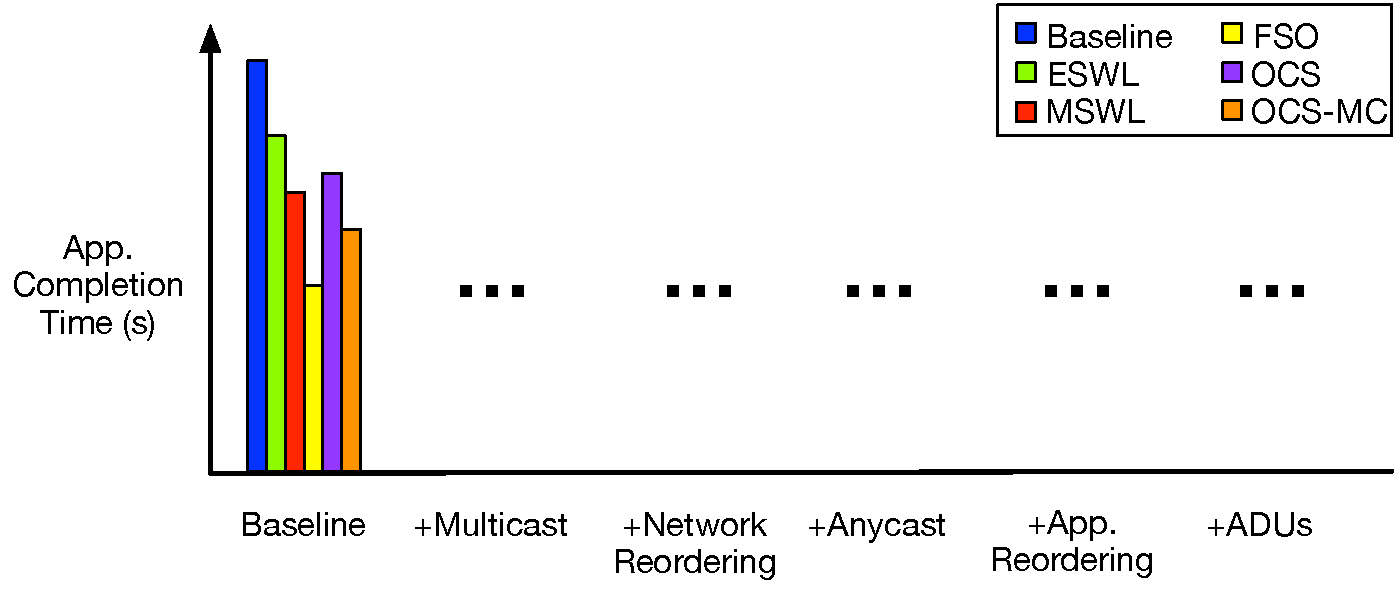
\includegraphics[width=0.47\textwidth]{figures/eval/map_red}
\caption{MapReduce-style Workload.}
\label{fig:eval_MR}
\end{figure}

\subsection{MapReduce Workload}
\label{sec:eval_MR}

\TODO{TODO}





\begin{figure}[t!!!]
\centering
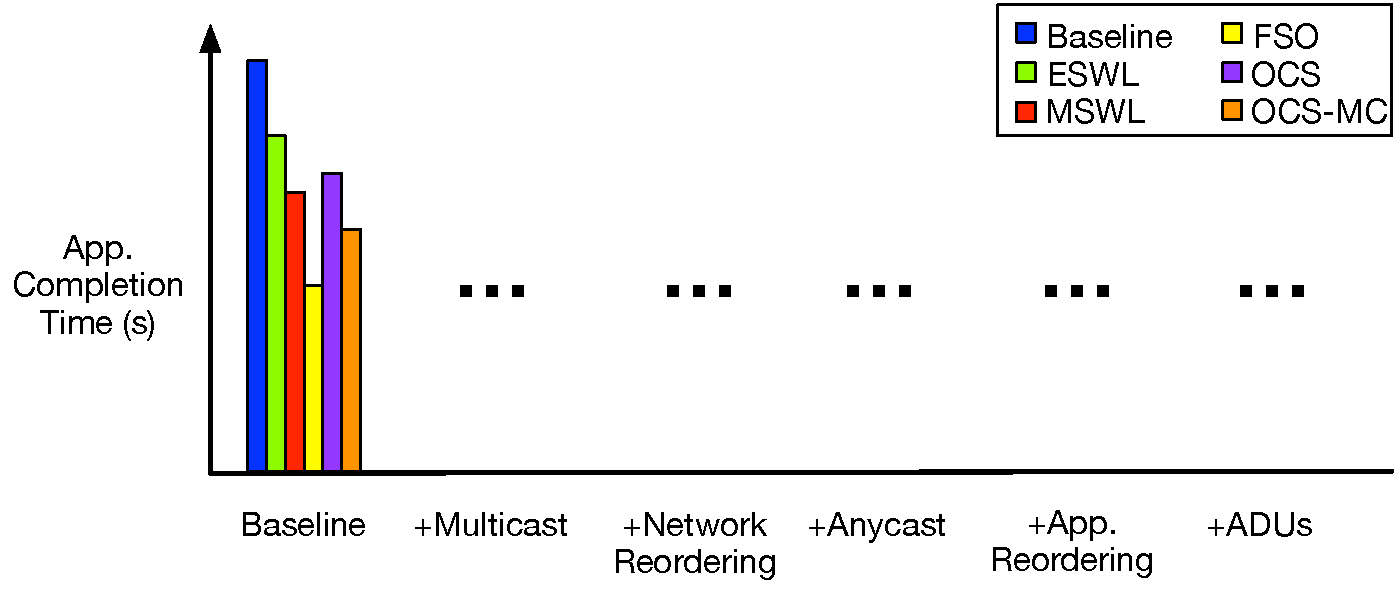
\includegraphics[width=0.47\textwidth]{figures/eval/map_red}
\caption{DFS-style Workload.}
\label{fig:eval_DFS}
\end{figure}

\subsection{DFS Workload}
\label{sec:eval_DFS}

\TODO{TODO}





\newpage\phantom{t}
\begin{figure}[t!!!]
\centering
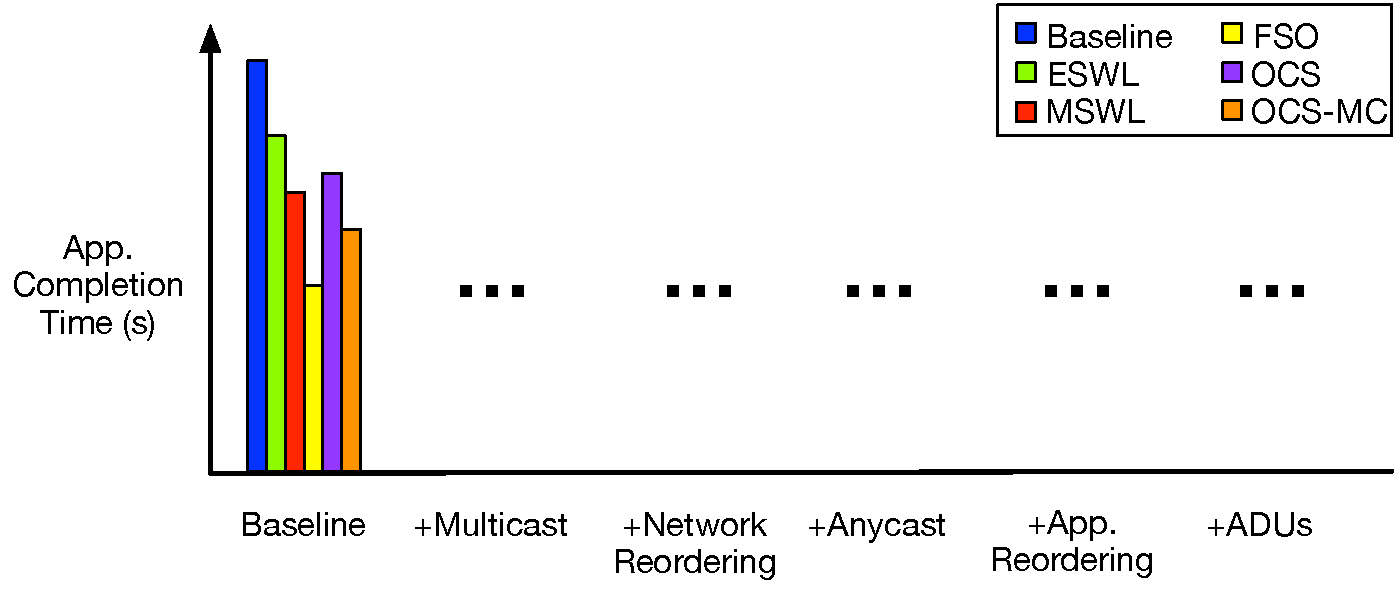
\includegraphics[width=0.47\textwidth]{figures/eval/map_red}
\caption{VM Migration-style Workload.}
\label{fig:eval_VM}
\end{figure}

\subsection{VM Migration Workload}
\label{sec:eval_VM}

\TODO{TODO}







\begin{figure}[t!!!]
\centering
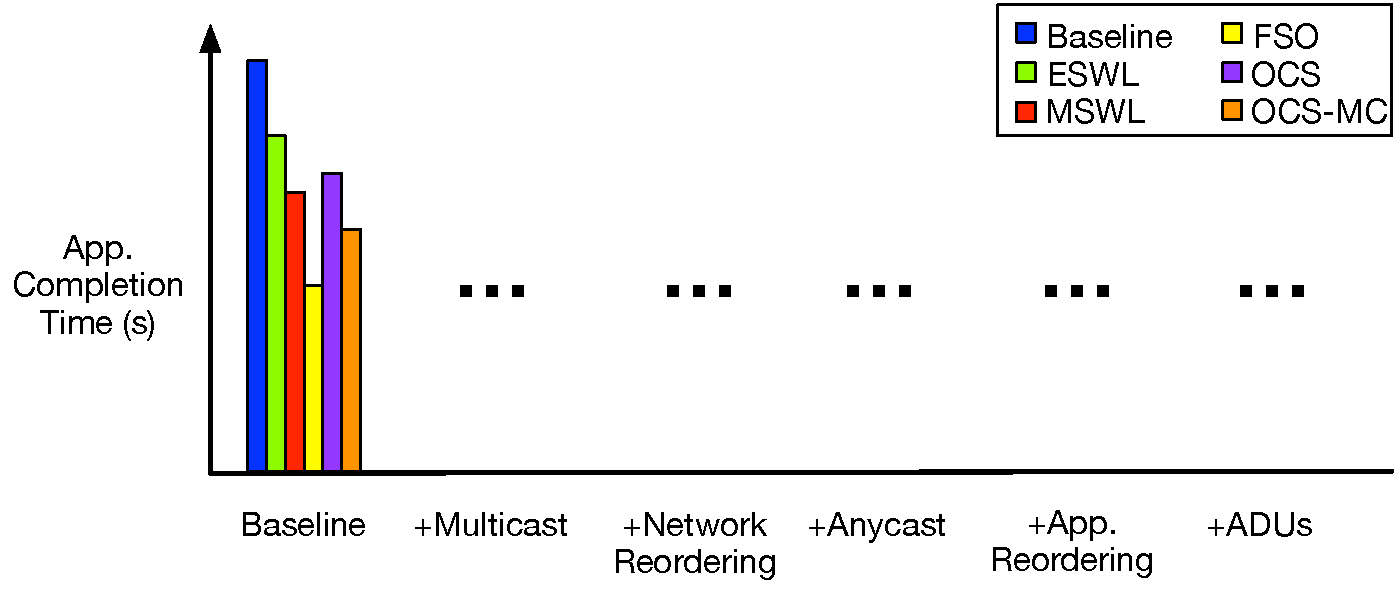
\includegraphics[width=0.47\textwidth]{figures/eval/map_red}
\caption{Search-style Workload.}
\label{fig:eval_search}
\end{figure}

\subsection{Search Workload}
\label{sec:eval_search}

\TODO{TODO}





\newpage\phantom{t}
\begin{figure}[t!!!]
\centering
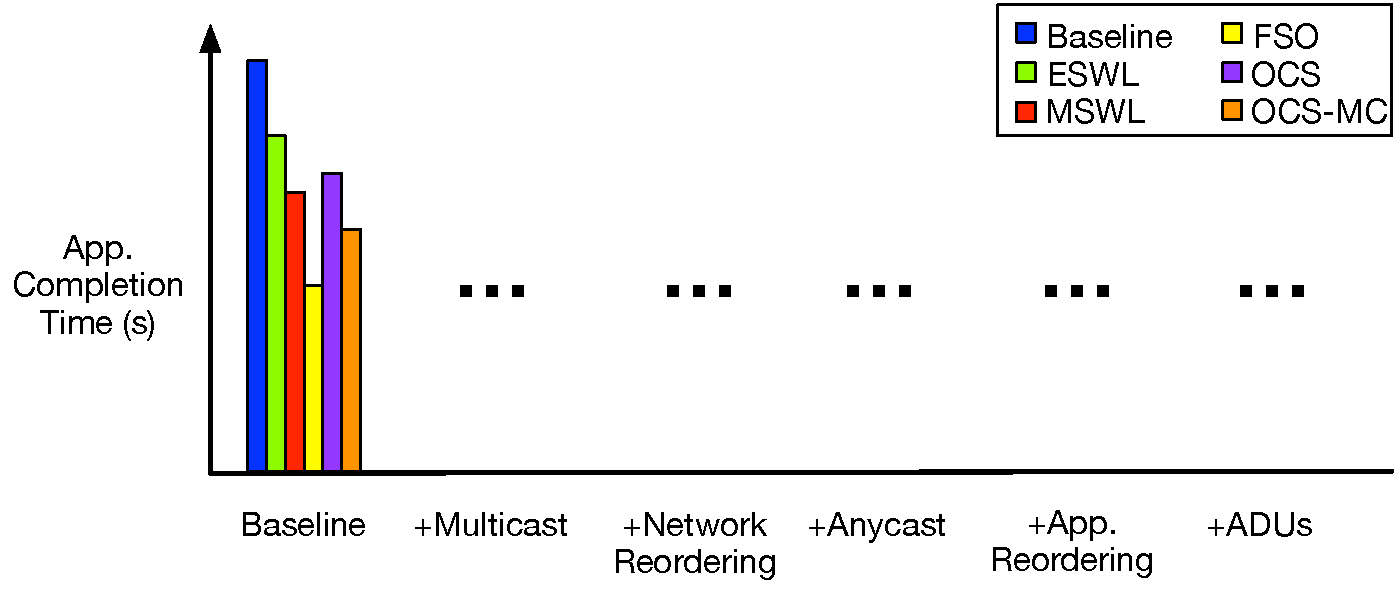
\includegraphics[width=0.47\textwidth]{figures/eval/map_red}
\caption{Combined VM Migration and Search Workload.}
\label{fig:eval_combined}
\end{figure}

\subsection{Combined Workload}
\label{sec:eval_combined}

\TODO{TODO}


\tightsection{Conclusion}
\label{sec:concl}



\newpage\phantom{t}
\bibliographystyle{acm}
\bibliography{ref}

\end{document}
